\chapter{Bilancio}
\section{Tipologie di imprese}

Le imprese possono essere suddivise in:
\begin{itemize}
    \item \textbf{Imprese profit} $\rightarrow$ svolgono un'attività economica con l'obiettivo di generare 
    un profitto per i proprietari o soci;
    \item \textbf{Imprese non profit} $\rightarrow$ perseguono principalmente finalità sociali, culturali 
    o di interesse collettivo e non hanno come obiettivo la distribuzione degli utili ai proprietari.
\end{itemize}

\subsection{Fatturato, ricavi e utile}
È importante distinguere tre concetti:
\begin{itemize}
    \item \textbf{Ricavi} $\rightarrow$ valore ottenuto dalla vendita di prodotti o dalla prestazione di servizi;
    \item \textbf{Fatturato} $\rightarrow$ valore complessivo delle vendite fatturate dall'impresa in un 
    determinato periodo;
    \item \textbf{Utile} $\rightarrow$ risultato economico positivo che rimane dopo aver sottratto ai 
    ricavi i costi sostenuti dall'impresa.
\end{itemize}

\[
\text{Utile} = \text{Ricavi} - \text{Costi}
\]

\noindent Ad esempio, un'impresa può avere un fatturato di 1 milione di euro ma un utile molto più basso, 
perché deve sostenere costi come stipendi, materie prime, affitti e altri costi di gestione.

\subsection{S.p.A. e S.r.l.}
La \textbf{S.p.A. (Società per Azioni)} è una società di capitali nella quale il capitale è suddiviso in 
\textbf{azioni}. È una forma societaria particolarmente adatta alle imprese di grandi dimensioni e permette più facilmente l'ingresso di numerosi investitori.
Le S.p.A. non sono obbligatoriamente quotate in borsa, ma possono esserlo se decidono di farlo.

\noindent La \textbf{S.r.l. (Società a responsabilità limitata)} è anch'essa una società di capitali, 
ma il capitale è suddiviso in \textbf{quote} e non in azioni. È generalmente utilizzata da imprese di dimensioni 
più contenute e presenta una struttura più semplice.

\noindent In entrambi i casi, i soci hanno generalmente una responsabilità limitata al capitale investito.

\noindent Dal punto di vista degli investimenti:
\begin{itemize}
    \item nella \textbf{S.p.A.} il capitale è rappresentato da azioni, rendendo generalmente più semplice 
    l'ingresso e l'uscita degli investitori;
    \item nella \textbf{S.r.l.} gli investitori acquistano quote della società e il trasferimento delle 
    partecipazioni è generalmente meno immediato.
\end{itemize}

\subsection{Stakeholder}
Gli \textbf{stakeholder} sono tutti i soggetti interessati all'attività e alle informazioni di un'impresa.

\noindent Alcuni esempi sono:
\begin{itemize}
    \item azionisti e soci;
    \item dipendenti;
    \item clienti;
    \item fornitori;
    \item banche e finanziatori;
    \item Stato e Pubblica Amministrazione.
\end{itemize}

\noindent Tra questi troviamo anche l'\textbf{Erario}, cioè l'insieme delle risorse finanziarie 
dello Stato. L'\textbf{Agenzia delle Entrate} è invece l'ente che si occupa principalmente della gestione e della riscossione dei tributi.

\subsection{Informazioni sulle imprese}
In Italia è possibile ottenere informazioni ufficiali sulle imprese attraverso il \textbf{Registro delle Imprese}. 
Uno degli strumenti utilizzabili per accedere a queste informazioni è \textbf{Telemaco}, attraverso cui è possibile consultare documenti 
come visure camerali e, quando disponibili, bilanci depositati.

\noindent Dai bilanci è possibile ricavare informazioni economiche e finanziarie sull'impresa, come ricavi, utile, costi, attività e debiti.

\subsection{Pagamento dei fornitori}
Nelle transazioni tra imprese il pagamento della merce non avviene necessariamente al momento della consegna. È comune concordare un pagamento 
differito, ad esempio a \textbf{30, 60 o 90 giorni}.

\noindent Questo significa che un'impresa può ricevere oggi la merce da un fornitore e pagarla successivamente secondo i termini stabiliti tra le parti.

\subsection{Tipologie di informazioni aziendali}
Le informazioni utilizzate da un'impresa possono essere suddivise in:
\begin{itemize}
    \item \textbf{Informazioni non quantitative} $\rightarrow$ informazioni che non vengono espresse attraverso valori numerici;
    \item \textbf{Informazioni quantitative} $\rightarrow$ informazioni espresse attraverso valori numerici.
\end{itemize}

\noindent Le informazioni quantitative si dividono a loro volta in:
\begin{itemize}
    \item \textbf{Informazioni monetarie} $\rightarrow$ espresse in termini economici e monetari;
    \item \textbf{Informazioni non monetarie} $\rightarrow$ espresse numericamente ma non in denaro, come quantità prodotte, ore lavorate o numero di dipendenti.
\end{itemize}

\noindent Le informazioni monetarie possono essere classificate in:
\begin{itemize}
    \item \textbf{Informazioni operative} $\rightarrow$ utilizzate per la gestione delle attività quotidiane;
    \item \textbf{Informazioni di bilancio} $\rightarrow$ descrivono la situazione economica, patrimoniale e finanziaria dell'impresa;
    \item \textbf{Informazioni per il management} $\rightarrow$ aiutano i manager a prendere decisioni e a controllare l'andamento dell'impresa;
    \item \textbf{Informazioni fiscali} $\rightarrow$ utilizzate per adempiere agli obblighi fiscali e tributari.
\end{itemize}
\begin{figure}[H]
    \centering  
    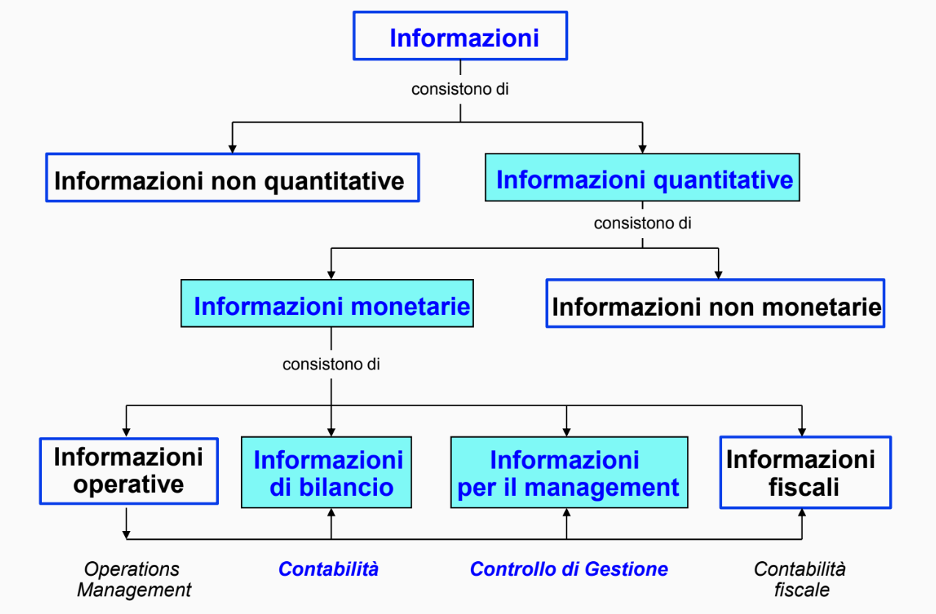
\includegraphics[width=0.7\linewidth]{../images/Infocazz.png}
    %\label{label}
\end{figure}
\subsection{Informazioni monetarie}
Le informazioni monetarie possono essere suddivise in quattro categorie:
\begin{enumerate}
    \item \textbf{Informazioni operative} $\rightarrow$ riguardano il dettaglio delle singole operazioni e sono necessarie per 
    lo svolgimento delle attività quotidiane dell'impresa;
    \item \textbf{Informazioni di contabilità} $\rightarrow$ vengono utilizzate dal management e da soggetti esterni e trovano 
    periodicamente una sintesi nel \textbf{Bilancio}, destinato anche alla pubblicazione;
    \item \textbf{Informazioni per il management} $\rightarrow$ vengono utilizzate per pianificare, prendere decisioni e controllare 
    l'andamento dell'impresa. Sono raccolte, analizzate e rendicontate attraverso il \textbf{Controllo di Gestione};
    \item \textbf{Informazioni di natura fiscale} $\rightarrow$ sono necessarie per determinare e pagare le imposte. Il reddito 
    imponibile viene determinato apportando specifiche rettifiche al risultato civilistico prima delle imposte.
\end{enumerate}
